\section{Introduction}
\label{sec:intro}


 \begin{figure*}
 	\center
 	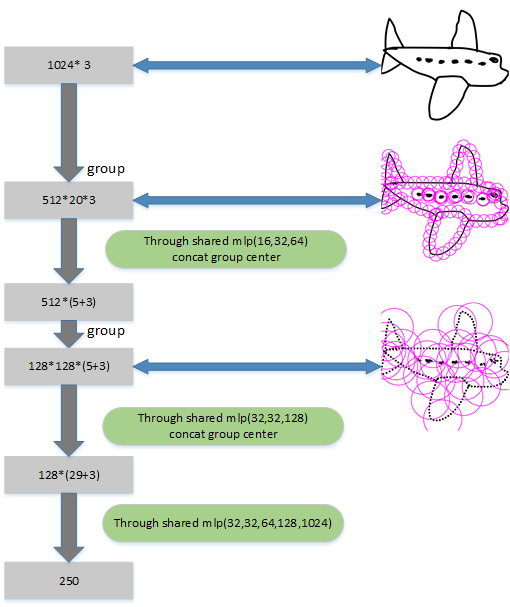
\includegraphics[width=\textwidth]{images/sketchpointnet.png}
 	\fcaption{SketchPointNet architecture. Given the input sketch, three mini PointNets are used to hierarchically extract features. Points are sampled along strokes and grouped in a bottom-up fashion. }
 	\label{fig:sketchpointnet}
 \end{figure*}


With the popularity of mobile and potable devices, sketching is getting easier for common users. As a powerful and effective tool for communication, freehand sketches have drawn a large amount of attention in image processing research.
Many approaches have been proposed for sketch recognition~\cite{Eitz2012HowDH, LiHSG15, Schneider2014SketchCA, Yu2015SketchaNetTB, Seddati2015DeepSketchDC, Dupont2016DeepSketch2D}.


%%%  Characteristic of freehand sketch
%While been drawn on 2D devices, freehand sketches can be naturally considered as a special type of digital images.
Freehand sketch possesses following unique characteristics, which make sketch recognition a challenging task, which is greatly different from natural image classification.
%
First, a sketch only contains extremely sparse visual signals as it is a very brief representation without any color or texture signals.
A large portion of pixels within a sketch image are blank.
%
Second, freehand sketches present large intra-class variance as sketches for the same object drawn by different users are extremely diverse.
The degree of shape distortions varies drastically from average users to professional artists.
%Because shape is the only hint that can be extracted from sketches, sketch recognition severely suffers from
%Moreover, the level of details is in a wide range, which makes the sketch recognition significantly challenging.
%
Third, the order of which the strokes are drawn in a sketch matters a lot, and thus provides temporal context for sketch recognition.
As claimed in previous research~\cite{Eitz2012HowDH}, sketches are typically drawn in a coarse-to-fine strategy. 
Details are usually added to the sketch later with short strokes.
Therefore, designing the technique for sketch classification should take the sparsity and temporal context into account.



%%% Earlier techniques
%
Ealier techniques for sketch recognition were mainly designed for recognizing hand-drawn numbers or letters~\cite{Hse2004SketchedSR, LaViola2004MathPad2AS, Fonseca2000UsingFL}.
Hse and Newton~\cite{Hse2004SketchedSR} used Zernike moments as features for sketches.
Laviola et al.~\cite{LaViola2004MathPad2AS} developed an approach for common mathematical symbol recognition.
Fonseca and Jorge~\cite{Fonseca2000UsingFL} designed geometrical features according to the profiles of stokes.
These approaches achieved good performance on handwritten symbols, which are simpler than sketches of common objects.
%Symbols from the same class usually have a standard template.
%
Eitz et al. \cite{Eitz2012HowDH} comprehensively analyzed the way of how human draw sketches, and published the TU-Berlin benchmark, a large dataset including 20000 sketches of 250 categories of objects.
This dataset is significantly challenging, and humans only achieve a $73.1\%$ recognition accuracy.
%
They extracted HOG features and used a support vector machine (SVM) for classification.
Other methods~\cite{LiHSG15, Schneider2014SketchCA} also extract hand-crafted features and use SVM classifiers.
However, for common objects, the representation capability of hand-crafted features is highly limited.


%%%%%% Deep learning methods

\para{CNN-based sketch recognition.}
With the great success of deep neural network (DNN) in natural image recognition, convolutional neural networks (CNN) have been applied to sketch recognition.
%While they convert freehand sketches into 2D images,
A certain number of existing approaches, such as Sketch-a-Net~\cite{Yu2015SketchaNetTB} and DeepSketch~\cite{Seddati2015DeepSketchDC},
straightforwardly convert freehand sketches into 2D images and exploit CNN to extract features for recognition from sketch images.
These CNN-based approaches achieve state-of-the-art performance on the challenging TU-Berlin benchmark.
%Compared to the deep networks for natural images, they have larger convolutional kernels and less convolutional layers.
%Although Sketch-a-Net \cite{Yu2015SketchaNetTB} and DeepSketch \cite{Seddati2015DeepSketchDC} achieve higher recognition accuracy than traditional methods.
However, regarding sketches as 2D pixel array, these CNN-based approaches require a large amount of network parameters to be learned.
%
As mentioned above, compared to natural images, freehand sketches are very sparse in 2D space. The data sparsity could greatly improve the network compactness.
Therefore, we adopt point-based DNN to design a compact network.

%%%%%%%%% Point-based deep networks
\para{Point-based DNNs.} Compared to CNN, the brand-new concept, which directly takes the discrete points as input, has been presented for point cloud processing recently~\cite{qi2017pointnet, qi2017pointnetplusplus, 1801.07791}.
The point-based DNN significantly reduces the model space and computational complexity.
%
PointNet~\cite{qi2017pointnet} presented the first deep network that directly consumes points for many applications of point clouds.
Its subsequent version, PointNet++~\cite{qi2017pointnetplusplus} used a hierarchical architecture to extract features from 3D point clouds for more robust recognition and segmentation.
%
Li et al.~\cite{1801.07791} proposed a $\chi$-transformation to permute unordered points into a latent potentially canonical order for feature learning.
While point-based networks were designed for point sets, they only exploits the spatial pattern.
In addition to spatial patterns, sketches contain temporal context, which is another important hint for recognition.
 %These networks consider only spatial pattern over the point clouds, while temporal pattern also plays an important role in sketch recognition.



In this paper, we propose a point-based deep network, named SketchPointNet, which takes advantages of both spatial and temporal pattern for efficient and robust sketch recognition.
%
Comparing with existing ConvNet-based sketch recognition approaches, we treat each sketch as a series of points, which is a sparser representation than images.
Comparing with the point-based DNNs, our SketchPointNet takes the stroke order into account.
%
By hierarchically extracting features from low level to the global level using three mini PointNets, the proposed SketchPointNet achieves comparable performance with state-of-the-art techniques on the challenging TU-Berlin dataset, and significantly reduces the number of network parameters.

